\chapter{Extended TROPOS Goal-oriented Software Development Methodology}\label{ch_proposal}

This section will describe our proposal with its application to the MPERS case study. Both TROPOS phases regarding requirements analysis will be fully presented, as long as the formal verification process that requires the runtime specification over the static system actor and also the additional contextual notation regarding context effects. The details about how a runtime goal model is translated to a probabilistic DTMC model in PRISM language will also be presented. Finally, the verification results of the selected dependability attributes will be discussed.

Further details about the TROPOS methodology may be found in the reference literature~[TROPOS]. This section will focus on the description of the novel approach for non-functional requirements verification of a runtime goal model through PMC technique.

\section{TROPOS Early Requirements Phase}

In Early Requirements phase, stakeholders are modelled as actors and their needs as goals. Each actor may be the depender or the dependee of a goal, task or a physical or information resource. Only the main system actor and the application domain stakeholders are analysed, leaving sub-systems and detailed agents analysis to later development phases.

The MPERS sytem and its social dependencies are presented by the actor model in Figure~\ref{fig:MPERS_ER}. System actors and social actors are displayed in different colors. Among the stakeholders, the Emergency Center represents a private or public organization that will provide the the emergency assistance service and product to patients. Patient and doctor respectively represent the assisted person and the medical responsible for defining new rules concerning the detection of emergency situations as part of an evolutionary and customized approach for emergency detection. Finally, sensors retailer should provide the vital signs sensors required by the system monitor.

\begin{figure*}[ht]
\centering
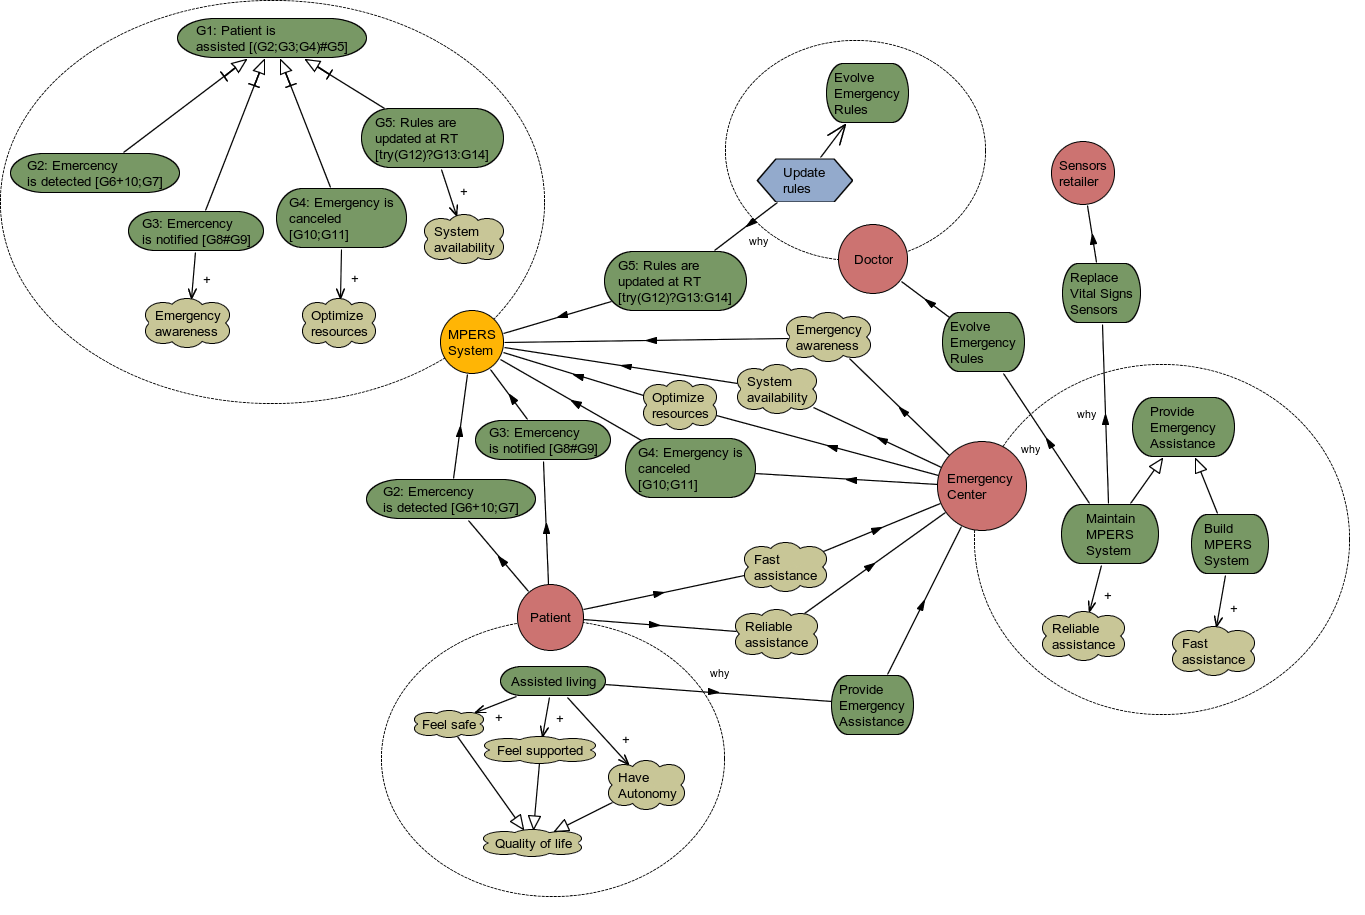
\includegraphics[width=1\textwidth]{imgs/MPERS_ER.png}
\caption{MPERS at TROPOS early requirements phase}
\label{fig:MPERS_ER}
\end{figure*}

From the diagram in Figure~\ref{fig:MPERS_ER} it is possible to have a first view of the MPERS system-to-be. Main goals are divided in detecting, notifying and cancelling an emergency. Also, the ability to update the emergency rules at runtime (RT) is the fourth and last mandatory goal (AND-decomposition) that fulfils the root `Patient is assisted' root goal. Functional system goals are strictly related to stakeholders functional and non-functional needs.

The yellow circle indicates that MPERS is a system actor. MPERS goals are already notated with a regex indicating its dynamic behaviour as part of the runtime goal model specification required by the proposal. This notation is a reflex of the late requirements phase, as the TAOM4E tool supporting TROPOS methodology shares unique entities and relations among different development phases. The regex syntax is enclosed by brackets to differentiate then from goal name. In future work a specific modelling compartment should receive the values for the runtime regex.

\section{TROPOS Late Requirements Phase}

Later requirements phase concentrates the analysis in the system-to-be and its operational environment. The MPERS goal model occupies the most part of the diagram and each of its main goals are further decomposed through AND/OR decomposition. Also, means-end tasks defines how leaf-goals are fulfilled and the runtime regex across goals and tasks specifies dynamic properties of the system-to-be behaviour. Figure~\ref{fig:MPERS_LR} illustrates the late requirements for the MPERS.

\begin{figure*}[h!]
\centering
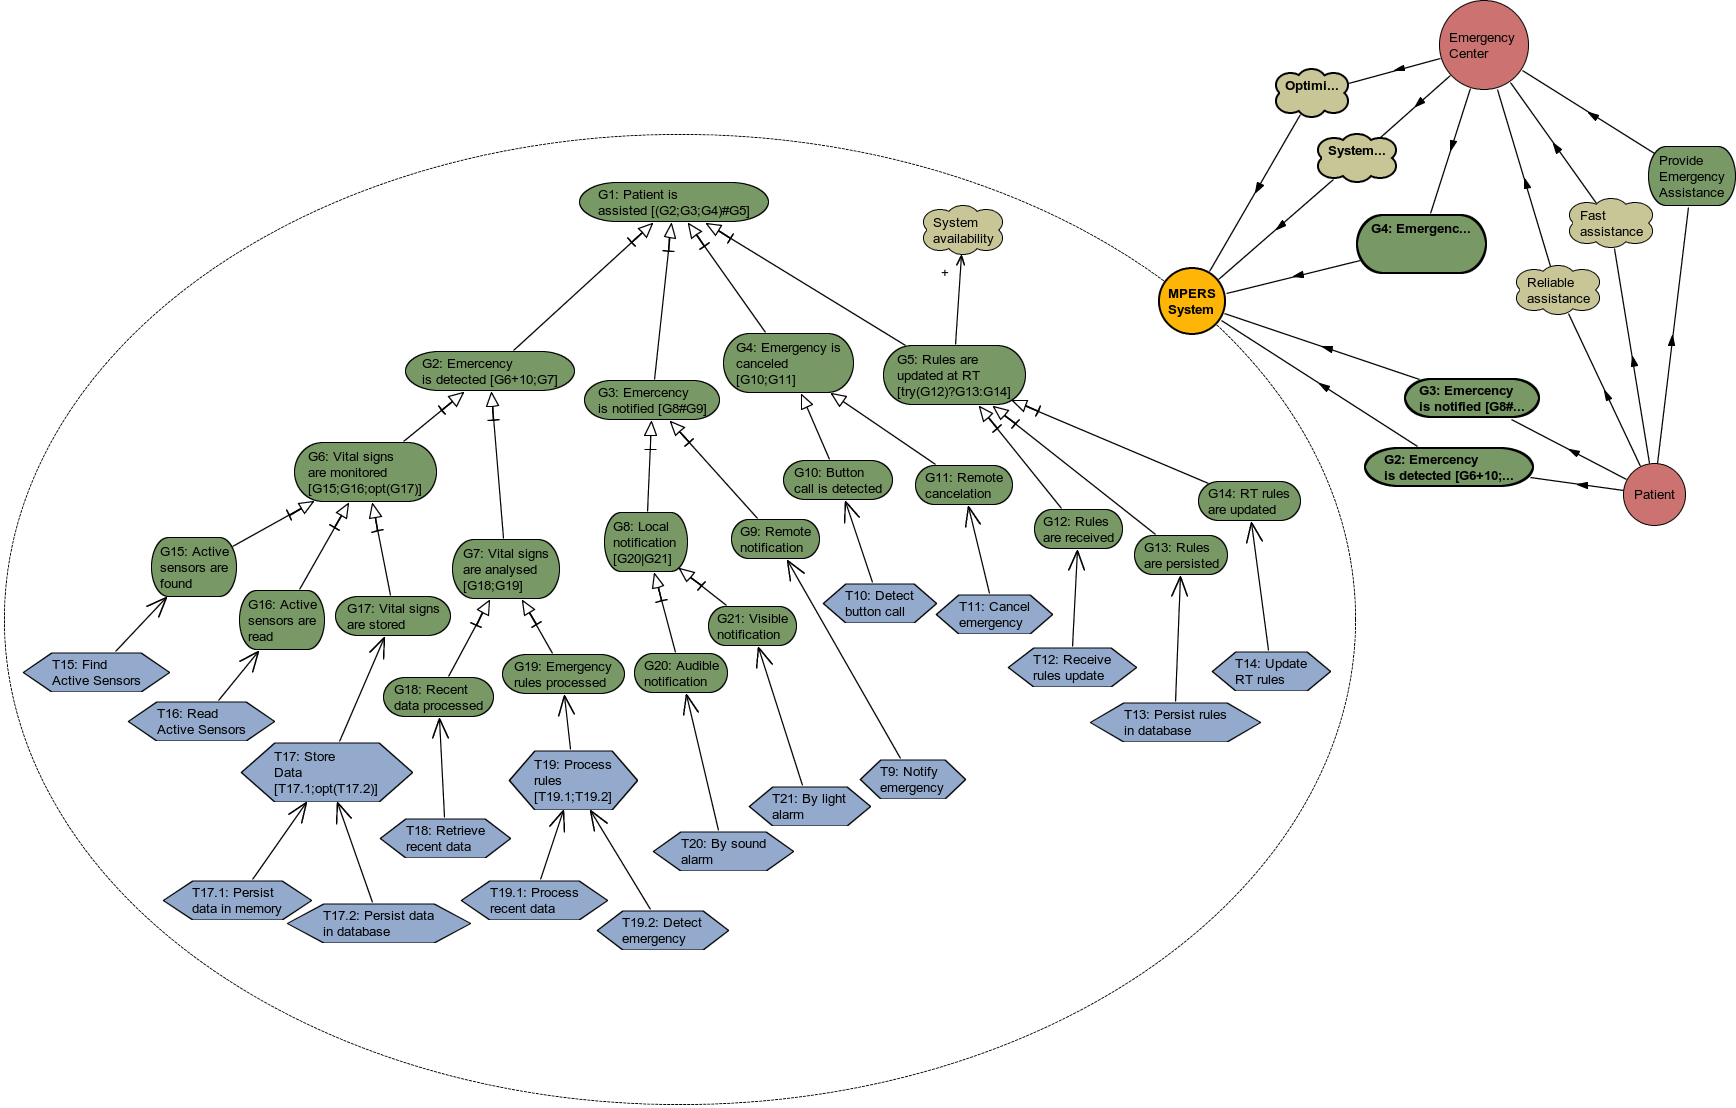
\includegraphics[width=1\textwidth]{imgs/MPERS_LR.png}
\caption{MPERS at TROPOS early requirements phase}
\label{fig:MPERS_LR}
\end{figure*}

At this point of the methodology, the system is represented as a monolithic actor and its goal model may be extended with the runtime specification. This extended model merges multiple views in the same diagram: strategical goals and operational tasks represent the requirements view for the system-to-be as well as the intentionality behind then, while the runtime specification provides a dynamic view of system operation through task execution.

A similar dynamic representation would be achieved by the direct correspondence between leaf-tasks of the model and the activities of an UML activity diagram. However, activity diagrams have an homogeneous granularity level and do not clearly correlate activities to the requirements they are meant to satisfy. Though activity diagrams are mostly graphical, the RGM representation mixes the original graphical goal model notation with a textual runtime regex. Its simple notation increases the value and utility of a goal model document. Figure~\ref{fig:MPERS_UMLAD} illustrates the similarity between the RGM and a corresponding UML activity diagram for the MPERS case study. 

\begin{figure*}[h!]
\centering
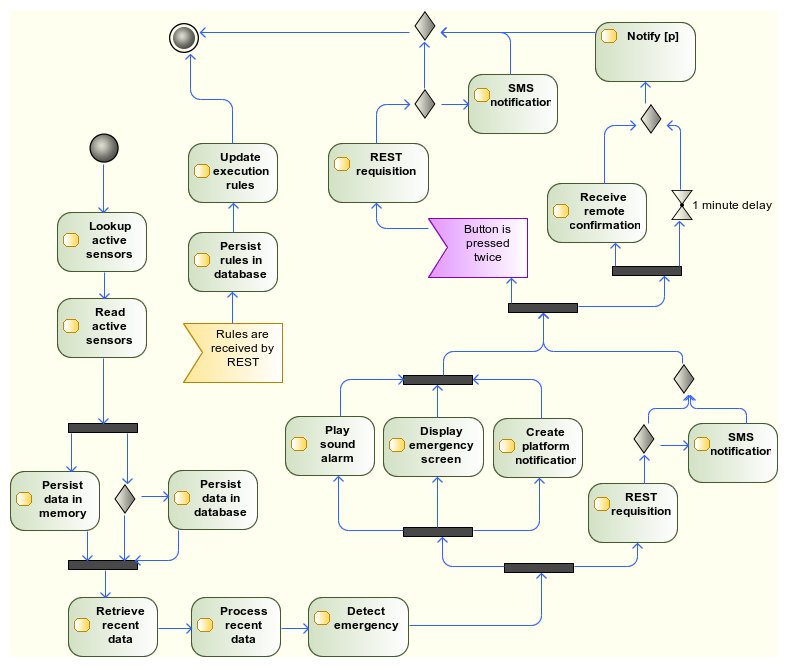
\includegraphics[width=1\textwidth]{imgs/MPERS_UMLAD.png}
\caption{MPERS tasks represented by a UML activity diagram}
\label{fig:MPERS_UMLAD}
\end{figure*}

RGM does not express that an emergency has to be confirmed after a time or event condition is met as the UML activity diagram is able to express. Both necessary and sufficient conditions for the triggering and fulfilment of goals and tasks are provided by Formal TROPOS language.  Still, sequential or parallel execution, alternative, optional and conditional flows as long as multiple executions of the same task can be expressed by the RGM, providing a rich behaviour specification that could be checked for meaningful non-functional requirements such as dependability attributes.

The idea of a runtime goal model is not to replace the activity diagrams, but to empower the goal model with a clear runtime syntax that could be employed in the conformance verification at both design time and during system execution and monitoring, as it was originally proposed. Depending on the complexity of the behaviour specification, a more robust runtime syntax would have to be employed or a standard UML behaviour specification such as activity or sequence diagrams would have to complement the goal model.

In our evaluation, we have first explored the use of the PMC technique for the verification of dependability attributes in the system model of the late requirements phase. The idea is to initially evaluate the approach in a monolithic representation of the system without the additional complexity of a multi-agent architecture. The evaluation involving later TROPOS phases should take place in future work. The remaining of this section will focus on the extended verification phase and TROPOS proposed by this work.

\section{TROPOS Extended Verification Phase}

To evaluate the current proposal with the MPERS case study, we have used the a discrete-time Markov chain (DTMC) probabilistic model and focused on the verification of NFR related to dependability, i.e., NFR that are either direct attributes encompassed by dependability or that are related to one or more of these attributes. Each NFR may be associated to a root level goal or to any decomposed subgoal. The correspondent PMC verification based on the execution of a set of tasks should be:

\begin{itemize}

\item \textit{Global verification}, if the set is a minimum set composed of the tasks that satisfies the chain of subgoals up to the root goal Gr.
\medskip

\item \textit{Local verification}, if the set is a minimum set composed of tasks that satisfies the chain of subgoals up to a goal Gx, where Gx != Gr.
\medskip

\end{itemize}

Given the possibility of a OR-decomposition in a goal model, more than one alternative can exist in terms of which subgoal should be fulfilled to satisfy its upper goal or which subtask should be performed to satisfy its upper task. Accordingly, both problem space (strategical goals) and solution space (means) may variate. 

The variability in the system goal model leads to more than one minimum set of tasks capable of fulfilling its local or root goals. Thus, either the analyst should decide which alternative will be verified by passing parameters values (deterministic alternative selection, or DAS) or the verification tool should decide based on some probabilistic distribution setted by the analysts (probabilistic alternative selection, or PAS).

DAS is useful for comparing system alternatives to decide which one should be used at design time based on the selected non-functional metrics. This approach is analogue to the TROPOS contribution analysis. In contrast, PAS provides verification for systems designed to operate in variable contexts, i.e., that may have to adapt. The verification of NFR metrics for these systems depend on the expected usage profile of different alternatives. 

As in the contextual goal model, contexts can limit which alternatives can be used in terms of goals and tasks. This effect must be included in the verification to have a realistic representation of the system. For this, analysts may decide which context will be verified (deterministic context selection, or DCS) and the corresponding adoptable alternatives are then checked using a DAS or PAS approach. Contexts values may also be selected following some distribution (probabilistic context selection, or PCS). Both approaches are complementary as the first will validate the system for an isolated context and the last offers a holistic system validation. Table~\ref{tab:DAS_PAS_DCS_PCS} following table summarizes the four approaches and their combination.

% Please add the following required packages to your document preamble:
% \usepackage{booktabs}
\begin{table}[h]
{\renewcommand{\arraystretch}{1.5}
\begin{tabularx}{\textwidth}{@{}l|XXX@{}}
\toprule
             &                                                         & \textbf{DAS}                                                                                                      & \textbf{PAS}                                                                                                     \\ \midrule
             &                                                         & A single alternative is selected by the analyst.                                                                  & Alternative selection follows a probabilistic distribution.                                                      \\
\textbf{DCS} & An unique context is selected by the analyst.           & Alternative selection by the analyst is limited by the selected context.                                          & Probabilistic alternative selection is limited by the selected context.                                          \\
\textbf{PCS} & Context selection follows a probabilistic distribution. & Alternative selection by the analyst may fail according to the probability of selecting an incomplatible context. & Probabilistic alternative selection may fail according to the probability of selecting an incomplatible context. \\ \bottomrule
\end{tabularx}
}
\caption{Description of the different approaches for verifying a system with variable alternatives and variable contexts.}
\end{table}

If the context selection is deterministic, there is no reason for selecting an alternative that is known to be incompatible with the selected context. In opposition, if context selection is probabilistic, that alternative may still be valid in other contexts. For instance, the alternative for identifying the patient location through GPS will certainly fail if the GPS signal is not available. Thus, the DAS-PCS combination leads to a reliability verification of one system alternative.

The same principle is applied to the PAS combinations. Incompatible alternatives are just not available for selection if the context is fixed. But if context selection is probabilistic, the probabilistic alternative selection should be limited to compatible context-alternative pairs. The PAS-PCS combination also can be used for reliability verification, as 






%This section is divided in preliminary conceptual explanation about the

In the PMC technique that has been adapted by this proposal, a behavioural specification, usually provided by UML activity and sequence diagrams, are manually converted to a probabilistic model in PRISM language. As a goal model is traversed from strategical root goal to operational leaf-goals, and each leaf-goal describes a desired state reachable by either a delegation to other actor or by a operational task, then a behaviour specification as proposed by the RGM may be consumed as input for the generation of probabilistic models in PRISM language.

Depending on the abstraction level and the nature of the verification, PRISM models may either very complex or may follow a clear pattern. For instance, modules can be used to represent leaf-tasks of a runtime goal model. Considering a DTMC model, a task workflow can be modelled as a sequence of probabilistic transitions of states in modules according to the execution order parsed from the RGM. The resulting model follows a pattern that was used to automatically generate PRISM models representing leaf-tasks execution directly from a runtime goal model.

The estimation of attributes through PMC technique is limited to those that a probabilistic model may evaluate. Dependability attributes have an abstract definition that must be associated to a concrete and verifiable PCTL property. To demonstrate our approach, we verify the MPERS model for the following attributes:

\begin{itemize}

\item \textbf{Reliability}, represented by the probability of a successful execution of all the activities involved in fulfilling leaf-goals of a certain system alternative. It is also know as the \textit{reachability} as the describes the probability of reaching a final and successful system state. 
\bigskip

\item \textbf{Availability}, represented by the power consumption estimation to maximize the time that the system will remain operational depending only on its battery. This attribute is well related to mobile computing. 
\medskip

\end{itemize}



must define the sequence of probabilistic state transitions in the model. These transitions 


each task has its own states, including the failure and the success states. Many factors may contribute to the correctness or the failure of system tasks, including internal and external events. The probability of a successful task execution defines its reliability. 

In a complex workflow of tasks with different rel 


 In order to be successful, tasks depend on the proper interaction among the components 

seen as an activity diagram and be used to generate a probabilistic model in PRISM language. This allows the model checking of the corresponding goal model as a set of activities for which temporal and other behaviour aspects are specified by the runtime regex of the RGM.

\section{Treating NFR Violations}

\begin{itemize}

\item Making a different choice for underlying components: In some cases the replacement of a technical component for another of the same class can improve the quality of how they achieve their goal. For instance,
\medskip

\item Behaviour optimization: The quality may also depend on the pattern used for the activities execution. The specification of a different pattern may eliminate the non-functional violation. 
\medskip

\item Contextualizing the alternative: An alternative may only violate a NFR in specific contexts. In this case, different valid alternatives may be used according to the context of operation.
\medskip

\item Alternative disposal: If the alternative is in absolute violation or if its validity is restricted to contexts that have at least one other valid alternative, this branch can be eliminated from the model.

\end{itemize}



Dependability analysis is used to provide information about different dependability attributes related to system failures. These metrics may be specified as non-functional requirements for isolated system functionalities or for the whole system. Instead of softgoals, we use meta-requirements over functional goals with clear-cut quantitative criteria such as `99.999\%' reliable - a probabilistic value to make it compatible with the PMC estimation results.

To perform the , we focus on dependability related metrics that should be estimated and compared to their required constraint values through quantitative analysis. Sensitive analysis to reveal how different system parts contribute to the overall value of those attributes. Sensitive analysis may be considered analogous to the original GORE contribution analysis.



\section{TROPOS to PMC Code Generation}

As we wanted to automate the code generating process for the verification model, the graphical modelling environment that supports TROPOS methodology and the code generation for multi-agents was extended to also generate probabilistic models for the PMC technique.

To reduce the effort of codifying the verification model, an automated generation of the PRISM probabilistic model was implemented based on an existing open source tool for TROPOS development support named TAOM4E[citation]. TAOM4E provides a graphical environment for goal modelling with TROPOS methodology based on the well known Eclipse Modelling Framework (EMF) and Graphical Editing Framework (GEF). The GORE to PRISM generator was implemented as a Eclipse plugin and integrated to the TAOM4E environment. 

The purpose  of the automated code generation for the probabilistic PRISM model is to optimize the formal verification step by abstracting the PRISM language from the analysts and reduce the overhead and time of the model verification. This should increase the feasibility of adopting the extended TROPOS methodology by keeping analysts with their original responsibility of modelling and analysing the system, its social environment and its different contexts of operation.






In terms of a high level system behaviour, each activity has its own states space including success and failure. Our probabilistic verification approach requires not only a formal specification of the system behaviour, but also metrics related to how individual components involved in system activities will perform in respect to the analysed metric. In reliability verification, each component has an individual probability of successfully performing its functional task. Analysts must obtain these values by consulting their manufacturer, by individually analysing each component reliability based on their behaviour specification until the atomic level or by monitoring these components in a testing or production environment. Further details of how individual metrics may be obtained for the PCM may be found at the literature and are out of the scope of this work.
